\documentclass[hyperref=unicode, presentation,10pt]{beamer}

\usepackage[absolute,overlay]{textpos}
\usepackage{array}
\usepackage{graphicx}
\usepackage{adjustbox}
\usepackage[version=4]{mhchem}
\usepackage{chemfig}
\usepackage[utf8]{inputenc}
\usepackage{caption}

\addtobeamertemplate{frametitle}{
	\let\insertframetitle\insertsectionhead}{}
\addtobeamertemplate{frametitle}{
	\let\insertframesubtitle\insertsubsectionhead}{}

\makeatletter
\CheckCommand*\beamer@checkframetitle{\@ifnextchar\bgroup\beamer@inlineframetitle{}}
\renewcommand*\beamer@checkframetitle{\global\let\beamer@frametitle\relax\@ifnextchar\bgroup\beamer@inlineframetitle{}}
\makeatother
\setbeamercolor{section in toc}{fg=red}
\setbeamertemplate{section in toc shaded}[default][100]

\usepackage{fontspec}
\usepackage{unicode-math}

\usepackage{polyglossia}
\setdefaultlanguage{czech}

\def\uv#1{„#1“}

\mode<presentation>{\usetheme{default}}
\usecolortheme{crane}

\setbeamertemplate{footline}[frame number]

\makeatletter
\setbeamertemplate{navigation symbols}{}


\title{Chemické pokusy - videa pro Commons}

\subtitle{Wikikonference 2024}
\author{Zdeněk Hugo Moravec \\ zdenek.moravec@wikimedia.cz}

\titlegraphic{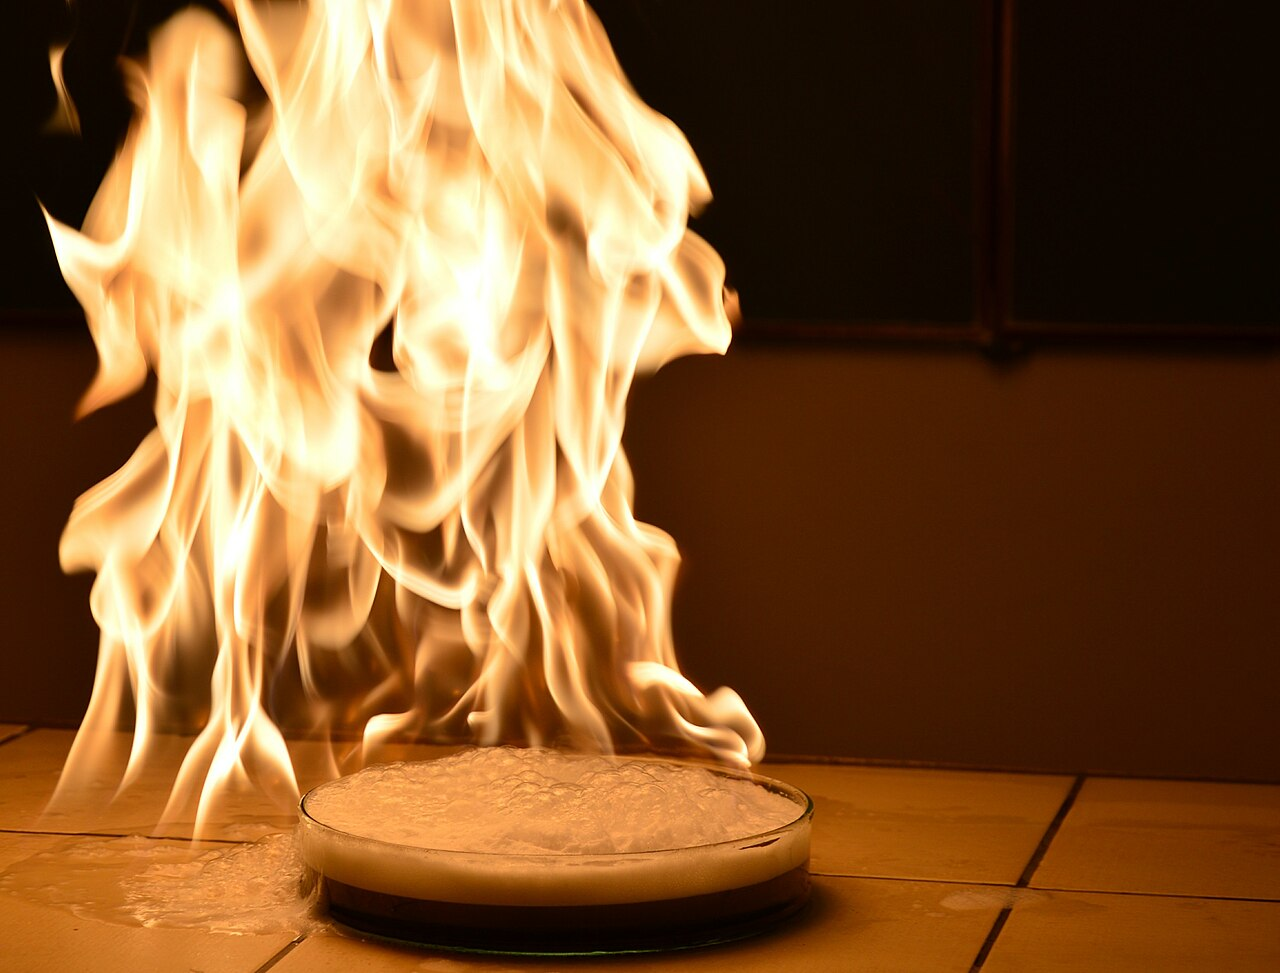
\includegraphics[height=.35\textheight]{img/intro.jpg}}

\date{}

\begin{document}

\begin{frame}
	\titlepage
\end{frame}

\section{Wikimedia Commons}
\frame{
	\frametitle{}
	\vfill
	\begin{columns}
	\begin{column}{.75\textwidth}
	\begin{itemize}
		\item Celkem více než 110 miliónů souborů (569 TB).\footnote[frame]{\href{https://commons.wikimedia.org/wiki/Special:MediaStatistics}{Wikimedia Commons -- Media statistics}}
		\item Obrázků je více než 101 miliónů (390 TB).
		\item Videí je pouze necelých 332 000 (30 TB).
	\end{itemize}
	\end{column}

	\begin{column}{.3\textwidth}
		\begin{figure}
			\adjincludegraphics[width=\textwidth]{img/Commons-logo.png}
		\end{figure}
	\end{column}
	\end{columns}
	\vfill
}

\section{Chemické pokusy}
\frame{
	\frametitle{}
	\vfill
	\begin{itemize}
		\item Pokusy jsou důležitým doplňkem výuky chemie, fyziky a dalších předmětů.
		\item Realizace složitějších experimentů je v prostředí základních a středních škol obtížná.
		\item Jako částečná náhrada mohou sloužit fotografie a videa.
		\item Výhodou zveřejnění videí na Commons, např. oproti Youtube, je jejich dostupnost pod licencí Creative Commons.
	\end{itemize}
	\vfill
}

\frame{
	\frametitle{}
	\vfill
	\begin{itemize}
		\item Samotné video nemůže obsahovat všechny informace potřebné pro správné pochopení pokusu, proto je vhodné doplnit zbylé informace do popisu videa nebo lépe např. do příslušné stránky na Wikipedii nebo Wikibooks.\footnote[frame]{\href{https://cs.wikibooks.org/wiki/Chemické_pokusy}{Chemické pokusy}}
	\end{itemize}

	\begin{figure}
		\adjincludegraphics[height=.55\textheight]{img/Wikibooks.png}
	\end{figure}
	\vfill
}

\frame{
	\frametitle{}
	\vfill
	\begin{itemize}
		\item Videa tvořím společně se SŠ a VŠ studenty v rámci:
		\begin{itemize}
			\item SOČ
			\item Bakalářských prací
			\item Diplomových prací
		\end{itemize}
		\item Pro natáčení je vhodné mít dostatečně kvalitní kameru (Logitech PTZ Pro) a příp. i mikrofon.
		\item Pro natáčení videí používáme OBS Studio\footnote[frame]{\href{https://obsproject.com/}{OBS Studio}} a pro stříhání Shotcut\footnote[frame]{\href{https://www.shotcut.org/}{Shotcut}}.
	\end{itemize}
	\begin{figure}
		\adjincludegraphics[height=.47\textheight]{img/lab.jpg}
	\end{figure}
	\vfill
}

\section{Ukázky pokusů}
\frame{
	\frametitle{}
	\vfill
	\textbf{Chemické pokusy}
	\begin{itemize}
		\item \href{https://cs.wikibooks.org/wiki/Chemick\%C3\%A9_pokusy/D\%C5\%AFkaz_uhl\%C3\%ADku_a_vod\%C3\%ADku_v_organick\%C3\%BDch_slou\%C4\%8Denin\%C3\%A1ch}{Důkaz uhlíku a vodíku v organických sloučeninách}
		\item \href{https://cs.wikibooks.org/wiki/Chemick\%C3\%A9_pokusy/Vznik_acetaldehydu_z_ethanolu}{Vznik acetaldehydu z ethanolu}
		\item \href{https://cs.wikibooks.org/wiki/Chemick\%C3\%A9_pokusy/T\%C3\%A1n\%C3\%AD_Woodova_kovu}{Tání Woodova kovu}
	\end{itemize}
	\vspace{3em}
	\textbf{Anorganická chemie}
	\begin{itemize}
		\item \href{https://cs.wikibooks.org/wiki/Anorganick\%C3\%A1_chemie/Tri\%C3\%A1da_\%C5\%BEeleza\%23\%C5\%BDeleznat\%C3\%A9_a_\%C5\%BEelezit\%C3\%A9_soli}{Příprava síranu železnatého (zelené skalice)}
		\item \href{https://commons.wikimedia.org/wiki/File:Reakce_oxidu_vanadi\%C4\%8Dn\%C3\%A9ho_s_hydroxidem_draseln\%C3\%BDm.webm}{Reakce oxidu vanadičného s hydroxidem draselným}
		\item \href{https://commons.wikimedia.org/wiki/File:Sr\%C3\%A1\%C5\%BEec\%C3\%AD_reakce_chloridu_\%C5\%BEeleznat\%C3\%A9ho_s_hydroxidem_draseln\%C3\%BDm_za_vzniku_hydroxidu_\%C5\%BEelezit\%C3\%A9ho.webm}{Srážení hydroxidu železitého}
		\item \href{https://commons.wikimedia.org/wiki/File:Sr\%C3\%A1\%C5\%BEec\%C3\%AD\%20reakce\%20s\%C3\%ADranu\%20\%C5\%BEeleznat\%C3\%A9ho_s_peroxidem.webm}{Oxidace železnatých solí peroxidem}
		\item \href{https://commons.wikimedia.org/wiki/File:Vlo\%C4\%8Dkov\%C3\%A1n\%C3\%AD.webm}{Vločkování}
	\end{itemize}
	\vfill
}

\section{Závěr}
\frame{
	\frametitle{}
	\vfill
	\centering \Huge
	\textbf{Děkuji za pozornost} \\[2ex]

	\large
	Zdeněk Hugo Moravec\\
	zdenek.moravec@wikimedia.cz \\
	\vfill
}

\end{document}
